\documentclass[11pt,harvard]{article}
\usepackage[letterpaper,top=1in, bottom=1in, left=1in, right=1in]{geometry}
\usepackage{graphicx}
\usepackage[sort]{natbib}
\usepackage{amssymb}
\usepackage{amsmath}
\usepackage{setspace}
\usepackage{url}
\usepackage{pdflscape}
\usepackage{longtable}
\usepackage{threeparttable, booktabs}
\usepackage[export]{adjustbox}
\usepackage{enumitem}
\usepackage{comment}
\usepackage{subcaption}
\usepackage{lmodern}
\usepackage[T1]{fontenc}
\usepackage{setspace} % Load the setspace package
\usepackage{parskip} % Load the parskip package
\usepackage{float}
\usepackage{subcaption}

\author{Nicole Wu  \and Cassandra Walker}
\date{\today}
\title{Gender and Food Security Reporting: Evidence from a Cross-over Experiment in Iraq}

\begin{document}
	\maketitle \vspace{-1cm}
	\onehalfspacing
	\pagebreak
	\setlength{\parskip}{6pt} % Set the desired space before and after paragraphs
	
% ------- 
\section{Introduction}

Food security assessment and reporting play a crucial role in the United Nations World Food Programme's (WFP) efforts to combat hunger and food insecurity. Given the significance of accurately measuring and interpreting food insecurity, particularly in situations where physical access is restricted during emergencies, it is imperative for WFP and its stakeholders to develop robust methodologies for this purpose.

Traditionally, WFP collects and analyzes food security data at the household level, and its program design and assistance are tailored to the household as a unit. However, it is important to recognize that there may be disparities in food security levels among different members within a household. In order to address this issue, the Needs Assessments and Targeting Unit at WFP RAM (RAM-N) and the Gender Equality Office (GEN) have collaborated to design a study that examines the intra-household differences in food security reporting.

The objective of this study is to shed light on the variations in food security experiences and perceptions among household members. By doing so, it aims to provide valuable insights for WFP and other relevant development agencies, helping them to adjust their operations during the assessment, planning, and implementation phases. Specifically, the study seeks to address gender inequality in food assistance and humanitarian responses, thereby facilitating more targeted and effective interventions.

Overall, this research endeavor holds the potential to enhance the understanding of intra-household dynamics related to food security reporting. Its findings can inform evidence-based decision-making within WFP and the broader development community, leading to improved gender-sensitive approaches to tackling food insecurity.

	\pagebreak
	
\subsection{Research Design}

In Iraq, the validation study of the remote Consolidated Approach for Reporting Indicators of Food Security (rCARI) involved a sample of 590 households. The selection of households was carried out using a specific sampling method, which should be detailed in this section of the paper. The households were selected from two internally displaced persons (IDP) camps and two refugee camps (NAMES AND DETAILS?). 

\emph{Data collection details to be added by Alirah} 
[Add sampling method and implementation details] The surveys were administered during a specific period, which should be mentioned in the paper. The implementation partner responsible for conducting the study should also be specified.

To ensure a comprehensive understanding of the intra-household dynamics, two interviews were conducted for each household - one with a male and one with a female member of the same household as a pair. Recruiting respondent of the opposite sex was typically based on the spouse or a household member with the smallest age difference from the primary respondent.

During the interviews, various aspects related to food security were assessed, including age, dietary diversity, coping strategies, and gender empowerment. These data were collected in-person from individual men and women within each household.

The sampling method used in the study rendered the analysis representative at a XX level. To provide a more comprehensive understanding, it is important to include additional details about the sampling method employed and the specific locations where the study was conducted. Additionally, it would be helpful to mention whether the camp registration system (such as SCOPE) was utilized to acquire the samples.

\emph{Do we want to introduce the remote survey here with the overall rCARI validation study design? } 


\subsection{Key Indicators}

\subsubsection{Minimum Dietary Diversity (MDD)}

The MDD Index, developed by the Food and Agriculture Organization of the United Nations (FAO) and the Food and Nutrition Technical Assistance III Project (FANTA), is a measurement tool used to assess the quality of an individual's diet. It incorporates ten food groups that reflect essential dimensions of diet quality and micro-nutrient adequacy. These food groups include:

\begin{enumerate}[label=\arabic*.]
	\item Staples: Foods made from grains, white roots and tubers, or plantains, including specialized nutritious foods (SNF) for women.
	\item Pulses: Beans, peas, and lentils.
	\item Nuts and seeds.
	\item Dairy products: Milk and milk products.
	\item Meat, poultry, and fish: Organ meats, red meat from mammals, processed meat, poultry and other white meats, fish, and seafood.
	\item Eggs from poultry or any other bird.
	\item Dark green leafy vegetables.
	\item Other vitamin A-rich fruits and vegetables, roots, and tubers.
	\item Other vegetables.
	\item Other fruits.
\end{enumerate}

In the survey, the MDD section is managed as a combination of 18 dichotomous questions (yes/no format), assessing whether adults consumed each of the food groups on the day prior to the survey. Typically, MDD is measured specifically for reproductive-aged women (referred to as MDDW). However, for this study, the aim is to analyze individual dietary diversity by the sex of the respondents.

By examining dietary diversity beyond reproductive-aged women, this study intends to explore potential differences in food consumption patterns and diet quality between different sexes. This approach allows for a broader understanding of dietary diversity within the sampled population, potentially uncovering variations and trends that may exist across different demographic groups.

Emphasizing the inclusion of both male and female respondents in the analysis of individual dietary diversity contributes to a more comprehensive examination of intra-household differences in food security reporting, particularly from a gender perspective.

\subsubsection{reduced Coping Strategies Index (rCSI)}

The study also aimed to determine if the rCSI results were influenced by the sex of the respondent. The rCSI is an indicator used to compare the hardship faced by households due to a shortage of food. As part of the WFP corporate CARI framework, the index measures the frequency and severity of the food consumption behaviors that households had to engage in due to food shortage in the seven days prior to the survey.

\begin{enumerate}[label=\arabic*.]
	\item Relied on less preferred, less expensive food
	\item Borrowed food or relied on help from friends or relatives
	\item Reduced the number of meals eaten per day
	\item Reduced portion size of meals
	\item Restricted consumption by adults in order for small children to eat 
	
\end{enumerate}

The gender-sensitive rCSI questions were developed specifically with the gender team. The questions aimed to determine, within the past seven days, who in the household applied the following strategies: The response options included: mainly adult male(s) or female(s), male or female children/youth, all adults equally, and all family members equally.

	\pagebreak
	
\subsection{Research Questions}
This study set out to answer the following questions:
\begin{itemize}
	\item Is the dietary diversity different for men and women of different households and inside the same household?
	\item Are rCSI results of the same households influenced by the respondent sex?
	\item Are the responses of newly developed gender-sensitive rCSI module influenced by the sex of respondents?
\end{itemize}
	\pagebreak
	
% ------- 
\section{Summary Statistics}

\subsection{Overall}

\begin{table}[htbp]
	\centering
	\begin{adjustbox}{max width=\textwidth}
		\begin{threeparttable}
			\caption{Summary Statistics of the Study Sample}
			\scriptsize
			%%% Table created in Stata by command iebaltab
%%% (https://github.com/worldbank/ietoolkit)
%%% (https://dimewiki.worldbank.org/iebaltab)
%%% The command was specified exactly like this: 
%%% iebaltab RESPAge RESPSex RESPPLW HHSize MDDIHHDisabledNb MDDIHHChronIllNb HHhostDisp FCS rCSI Lcs_Stress_Coping Lcs_Crisis_Coping Lcs_Emergency_Coping HHExpTotal, grpvar(Status) nonote total replace format(%12.2fc) grplabels(1 IDP @ 2 Refugee) onerow rowvarlabels savetex("/Users/nicolewu/Library/CloudStorage/OneDrive-WorldFoodProgramme/2_CARI_validation/1_rCARI_study/1_Pilot_country/1_Iraq/9_Analysis/8_Manuscript/2_tables/Summary_Stats_All_no_Group.tex")

\begin{tabular}{@{\extracolsep{5pt}}lcccc}
\\[-1.8ex]\hline \hline \\[-1.8ex]
 & \multicolumn{1}{c}{(1)}  & \multicolumn{1}{c}{(2)}  & \multicolumn{1}{c}{(3)}  & \multicolumn{1}{c}{(2)-(3)} \\
 & \multicolumn{1}{c}{Total}  & \multicolumn{1}{c}{IDP}  & \multicolumn{1}{c}{Refugee}  & \multicolumn{1}{c}{Pairwise t-test}  \\
Variable & Mean/(SE) & Mean/(SE) & Mean/(SE) & Mean difference \\ \hline \\[-1.8ex] 
Respondent Age   & 38.68    & 37.89    & 39.54    & -1.65   \\
 & (0.50)  & (0.73)  & (0.69)  &  \\ [1ex]
Sex of the respondent   & 0.48    & 0.57    & 0.37    & 0.20***   \\
 & (0.02)  & (0.03)  & (0.03)  &  \\ [1ex]
Pregnant or Lactating Respondent   & 0.08    & 0.04    & 0.13    & -0.09***   \\
 & (0.01)  & (0.01)  & (0.02)  &  \\ [1ex]
Household Size   & 5.78    & 5.96    & 5.59    & 0.38*   \\
 & (0.10)  & (0.16)  & (0.12)  &  \\ [1ex]
Number of disabled household members   & 0.25    & 0.27    & 0.22    & 0.05   \\
 & (0.02)  & (0.03)  & (0.04)  &  \\ [1ex]
Number of household members with chronic disease   & 0.62    & 0.40    & 0.87    & -0.47***   \\
 & (0.03)  & (0.03)  & (0.05)  &  \\ [1ex]
Household currently hosting IDP or Refugee   & 0.17    & 0.02    & 0.34    & -0.32***   \\
 & (0.02)  & (0.01)  & (0.03)  &  \\ [1ex]
Food Consumption Score   & 61.86    & 62.77    & 60.88    & 1.89   \\
 & (0.70)  & (1.04)  & (0.91)  &  \\ [1ex]
Reduced Consumption Strategies Index (rCSI)   & 14.36    & 12.90    & 15.95    & -3.06***   \\
 & (0.52)  & (0.62)  & (0.83)  &  \\ [1ex]
Household engaged in stress coping strategies   & 0.89    & 0.88    & 0.90    & -0.03   \\
 & (0.01)  & (0.02)  & (0.02)  &  \\ [1ex]
Household engaged in crisis coping strategies   & 0.70    & 0.72    & 0.67    & 0.06   \\
 & (0.02)  & (0.03)  & (0.03)  &  \\ [1ex]
Household engaged in emergency coping strategies   & 0.09    & 0.12    & 0.06    & 0.06**   \\
 & (0.01)  & (0.02)  & (0.01)  &  \\ [1ex]
Monthly total household expenditure   & 646,055.31    & 616,489.57    & 678,128.41    & -61,638.84*   \\
 & (15,848.78)  & (20,260.02)  & (24,567.83)  &  \\ [1ex]
\hline \\[-1.8ex]
Number of observations  & 590   & 307   & 283  & 590  \\
\hline \hline \\[-1.8ex]

\end{tabular}
 
			\label{tab:Summary_Stats_All_no_Group}
			\begin{tablenotes}[para,flushleft]
				\item Note: Significance: * p$<$0.10, ** p$<$0.05, *** p$<$0.01. 
			\end{tablenotes}
		\end{threeparttable}
	\end{adjustbox}
\end{table}

\subsection{rCSI Matched Pairs}

\subsection{First Survey F2F vs. Remote}

	\pagebreak
	
% ------- 
\section{MDD}

For primary respondents ($n=431$), consisting of 193 households with female primary respondents and 238 households with male respondents, the overall averages for MDD appear similar, with an average of 5.1 for women and 5.2 for men. 

\begin{figure}[H]
	\caption{MDD Index for Original Respondents: Female vs. Male} \label{fig:Iraq_MDD_Index_F2F_Original_Gender}
	\begin{center}
		
\includegraphics[scale=.4]{1_figures/Iraq_MDD_Index_F2F_Original_Gender.png}
	\end{center}
	\footnotesize
	Note: Significance: * p$<$0.10, ** p$<$0.05, *** p$<$0.01. Original respondents n = 431 (Female = 238, Male = 193)  	
\end{figure}

However, when we analyze the responses by food consumption groups or households with acceptable Food Consumption Score (FCS) ($n=381$) and households with poor/borderline FCS ($n=50$), we observe differences in responses based on the sex of the respondents, particularly within the poor/borderline FCS group. In the poor/borderline FCS category, males scored higher on dietary diversity compared to female respondents (5.3 for males compared to 4.1 for females). On the other hand, within the acceptable FCS category, females scored better than males (5.4 vs. 5.0).

\begin{figure}[H]
	\caption{MDD Index for Original Respondents: Female vs. Male by FCG} \label{fig:Iraq_MDD_Index_F2F_Original_Gender_FCG}
	\begin{center}
		
\includegraphics[scale=.4]{1_figures/Iraq_MDD_Index_F2F_Original_Gender_FCG.png}
	\end{center}
	\footnotesize
	Note: Significance: * p$<$0.10, ** p$<$0.05, *** p$<$0.01. 
	Original respondents n = 431 (Female = 238, Male = 193).
	FCG = Food Consumption Groups
\end{figure}

In the paired sample of 303 households, the average MDD of women was 4.8, while the average MDD for men was 4.7.

\begin{figure}[htbp]
	\centering
	\caption{Comparison of Intra-Household MDD Categories}
	\begin{subfigure}{0.49\columnwidth} % Adjust the width as needed
		\centering
		\caption{I Female and Male Mean}
		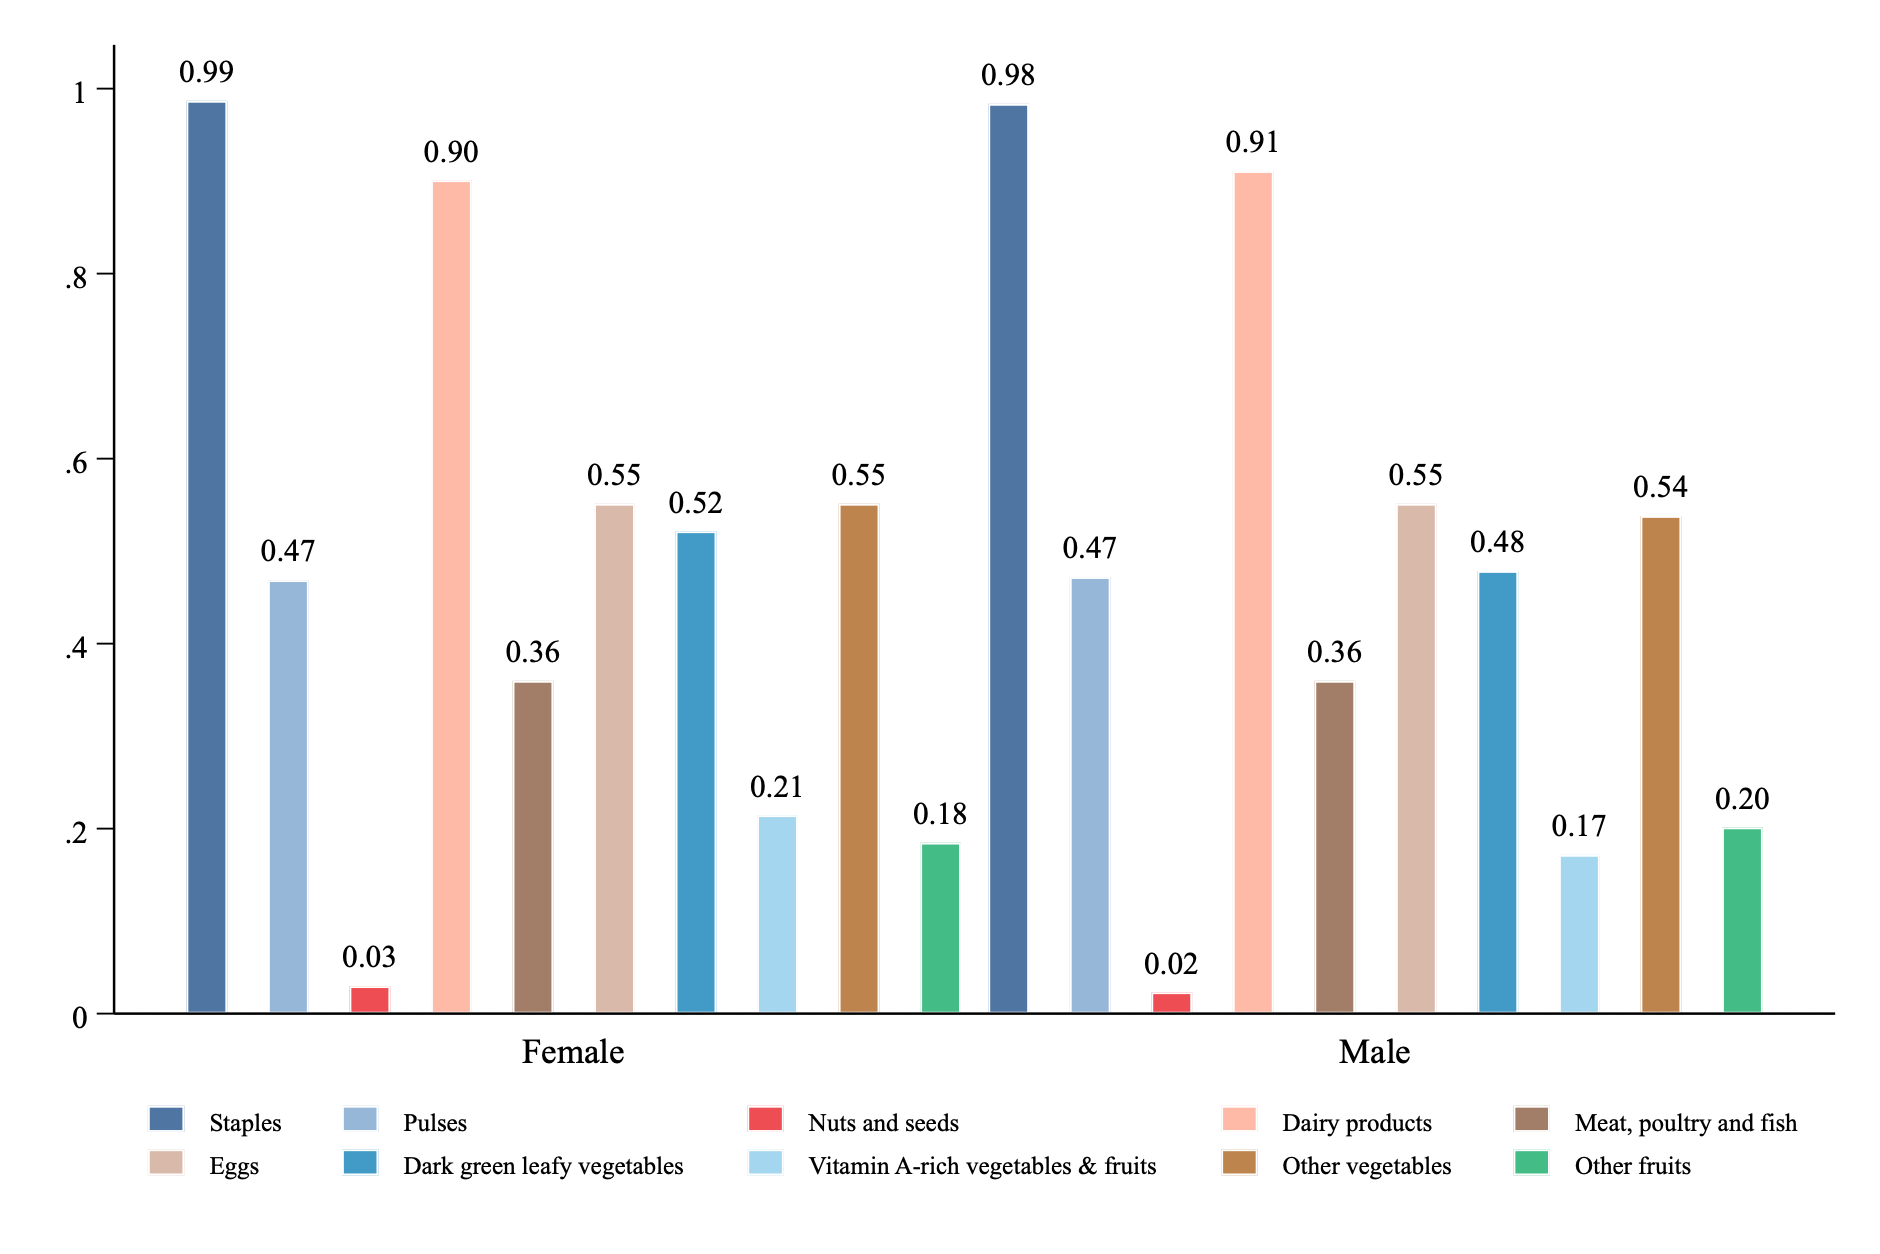
\includegraphics[width=\linewidth]{1_figures/Iraq_MDD_F2F_Gender_Summary.png}
		\label{fig:Iraq_MDD_F2F_Gender_Summary}
	\end{subfigure}
	\hfill
	\begin{subfigure}{0.49\columnwidth} % Adjust the width as needed
		\centering
		\caption{Female - Male Difference}
		
\includegraphics[width=\linewidth]{1_figures/Iraq_MDD_F2F_Gender_Comparison.png}
		\label{fig:Iraq_MDD_F2F_Gender_Comparison}
	\end{subfigure}
	\footnotesize
	Note: Significance: * p$<$0.10, ** p$<$0.05, *** p$<$0.01.
	Matched household pairs N = 303
\end{figure}


\begin{figure}[H]
	\caption{Intra-Household MDD Categories by FCG: Female - Male Difference} \label{fig:Iraq_MDD_F2F_Gender_Comparison_FCG}
	\begin{center}
		
\includegraphics[scale=.3]{1_figures/Iraq_MDD_F2F_Gender_Comparison_FCG.png}
	\end{center}
	\footnotesize
	Note: Significance: * p$<$0.10, ** p$<$0.05, *** p$<$0.01.
	Matched household pairs N = 303 (FCS Poor or Borderline N = 33; FCS Acceptable N = 270)
\end{figure}


\begin{figure}[H]
	\caption{Intra-Household MDD Index by FCG: Female - Male Difference} \label{fig:Iraq_MDD_Index_F2F_Gender_FCG}
	\begin{center}
		
\includegraphics[scale=.3]{1_figures/Iraq_MDD_Index_F2F_Gender_FCG.png}
	\end{center}
	\footnotesize
	Note: Significance: * p$<$0.10, ** p$<$0.05, *** p$<$0.01.
	Matched household pairs N = 303 (FCS Poor or Borderline N = 33; FCS Acceptable N = 270)
\end{figure}


\begin{table}[htbp]
	\centering
	\begin{adjustbox}{max width=\textwidth}
		\begin{threeparttable}
			\caption[Paired Gender Difference for MDD]{Paired Gender Difference for MDD}
			\scriptsize
			{
\def\sym#1{\ifmmode^{#1}\else\(^{#1}\)\fi}
\begin{tabular}{l*{1}{cccc}}
\hline\hline
&     Female Mean&   Male Mean&Diff: Female - Male&     P Value\\
\hline
\textbf{\textit{Original Food Categories:}}&       &       &       &\\
StapCer     & 0.99  & 0.98  & 0.00  & 0.71 \\
StapRoo     & 0.45  & 0.44  & 0.00  & 0.86\\
	Pulse       & 0.47  & 0.47  & -0.00 & 0.87\\
	Nuts        & 0.03  & 0.02  & 0.01  & 0.53\\
	Milk        & 0.22  & 0.22  & -0.00 & 0.80\\
	Dairy       & 0.84  & 0.84  & -0.00 & 0.87\\
	PrMeatO     & 0.03  & 0.04  & -0.01 & 0.21\\
	PrMeatF     & 0.03  & 0.04  & -0.01 & 0.16\\
	PrMeatPr    & 0.00  & 0.01  & -0.00 & 0.56\\
	PrMeatWh    & 0.31  & 0.31  & 0.01  & 0.68\\
	PrFish      & 0.04  & 0.03  & 0.01  & 0.26\\
	PrEgg       & 0.55  & 0.55  & 0.00  & 1.00\\
	VegGre      & 0.52  & 0.48  & 0.04  & 0.05**\\
	VegOrg      & 0.20  & 0.17  & 0.04  & 0.05*\\
	FruitOrg    & 0.03  & 0.02  & 0.02  & 0.13\\
	VegOth      & 0.55  & 0.54  & 0.01  & 0.55\\
	FruitOth    & 0.18  & 0.20  & -0.02 & 0.40\\
	Snf         & 0.00  & 0.00  & 0.00  & . \\
	\textbf{\textit{Standardized MDD Food Categories:}}&       &       &       &\\
	Staples     & 0.99  & 0.98  & 0.00  & 0.71\\
	Pulses      & 0.47  & 0.47  & -0.00 & 0.87\\
	NutsSeed    & 0.03  & 0.02  & 0.01  & 0.53\\
	Dairies     & 0.90  & 0.91  & -0.01 & 0.55\\
	MeatFish    & 0.36  & 0.36  & 0.00  & 1.00\\
	Eggs        & 0.55  & 0.55  & 0.00  & 1.00\\
	LeafGVeg    & 0.52  & 0.48  & 0.04  & 0.05**\\
	VitA        & 0.21  & 0.17  & 0.04  & 0.04**\\
	OtherVeg    & 0.55  & 0.54  & 0.01  & 0.55\\
	OtherFru    & 0.18  & 0.20  & -0.02 & 0.40\\
	MDD Index   & 4.77  & 4.69  & 0.08  & 0.21\\
	MDD Index 5 & 0.50  & 0.49  & 0.01  & 0.65\\
\hline\hline
\end{tabular}
}

 
			\label{tab:Iraq_MDD_F2F_Gender_Difference_Paired_ttest}
			\begin{tablenotes}[para,flushleft]
				\item Note: Significance: * p$<$0.10, ** p$<$0.05, *** p$<$0.01. 
			\end{tablenotes}
		\end{threeparttable}
	\end{adjustbox}
\end{table}

\pagebreak

% ------- 
\section{rCSI}

\pagebreak
	
\end{document}

